\documentclass[aspectratio=169]{beamer}
\usepackage[russian]{babel}
\usepackage[utf8]{inputenc}
\usepackage{verbatim}
\usepackage{graphicx}
\usepackage{pgfpages}
\usepackage{ulem}
\usepackage{float}
\usepackage{amsmath}

\setbeamercolor{title}{fg=white}
\setbeamercolor{author}{fg=white}
\setbeamercolor{normal text}{fg=black}
\setbeamercolor{frametitle}{fg=black}
\setbeamercolor{item}{fg=red}
\setbeamercolor{block title}{fg=red}
\setbeamercolor{section in toc}{fg=red}
\setbeamercolor{footline}{fg=white}
\setbeamercolor{title in head/foot}{fg=white,bg=black}

\setbeamertemplate{navigation symbols}{}
\setbeamertemplate{headline}{
    
\includegraphics[height=1mm, width=\paperwidth]{wg-headline.png}
}

\setbeamertemplate{footline}{
    \begin{beamercolorbox}[ht=1.2em]{title in head/foot}
        {\footnotesize \hspace{1em}\inserttitle: \insertshortauthor}
    \end{beamercolorbox}
}

\begin{document}

\title{World of Tanks: несколько идей из опыта разработки}
\author{Максим Мельников}
\date{}

{

\title{
    
\includegraphics[width=0.4\textwidth]{wg-logo.png}\\
    {\LARGE WORLD OF TANKS\\НЕСКОЛЬКО ИДЕЙ ИЗ ОПЫТА РАЗРАБОТКИ}
}
\author{МАКСИМ МЕЛЬНИКОВ}

\usebackgroundtemplate{
\includegraphics[width=\paperwidth]{wg-end.jpg}}
\begin{frame}[plain]{}
    \titlepage
\end{frame}

}

\usebackgroundtemplate{
\includegraphics[width=\paperwidth]{wg-bg.jpg}}

\begin{frame}{КТО Я}
    \begin{itemize}
        \item Wargaming.net
            \begin{itemize}
                \item \sout{Order of War}
                \item \sout{Order of War: Challenge}
                \item World of Tanks developer
            \end{itemize}
        \item Linux Mobile hobbyist
            \begin{itemize}
                \item \sout{Openmoko}
                \item systemd
                \item telepathy
                \item Gentoo
            \end{itemize}
    \end{itemize}
\end{frame}

\begin{frame}{WORLD OF TANKS СЕГОДНЯ}
    \begin{itemize}
        \item 800k одновременно играющих в пике
        \item 8M сообщений в секунду
        \item 300 серверов для обслуживания игры
        \item 60M посещений игрового портала в месяц
        \item 5PB (петабайт) на установку и обновления игрового клиента в месяц
    \end{itemize}
\end{frame}

\begin{frame}{АРХИТЕКТУРА WORLD OF TANKS}
    \begin{itemize}
        \item клиент игры --- тонкий клиент, плеер
        \item сервер --- расчёт игрового мира
        \item кластер --- сотни процессов работающих как единое целое (сервер)
        \item игровой мир --- пошаговый, шаги очень маленькие
    \end{itemize}
\end{frame}

\begin{frame}{АРХИТЕКТУРА КЛАСТЕРА}
    \begin{columns}

    \begin{column}{0.33\textwidth}
    \begin{block}{Storage*}
        \begin{itemize}
            \item MySQL
            \item MySQL*
            \item RabbitMQ
        \end{itemize}
    \end{block}
    \end{column}

    \begin{column}{0.33\textwidth}
    \begin{block}{Nodes}
        \begin{itemize}
            \item BaseApp
            \item CellApp
            \item LoginApp
        \end{itemize}
    \end{block}
    \end{column}

    \begin{column}{0.33\textwidth}
    \begin{block}{Managers}
        \begin{itemize}
            \item BaseAppMgr
            \item CellAppMgr
            \item DbMgr
        \end{itemize}
    \end{block}
    \end{column}

    \end{columns}
    \vspace*{1cm}
\end{frame}

\begin{frame}{АРХИТЕКТУРА КЛАСТЕРА II}
    \begin{columns}
        \begin{column}{0.4\textwidth}
        \begin{block}{BaseApp}
        \begin{itemize}
            \item Account
            \item ChatChannel
            \item Clan
            \item Admin
            \item SysMessenger
            \item Node
        \end{itemize}
        \end{block}
        \end{column}

        \begin{column}{0.4\textwidth}
        \begin{block}{CellApp}
        \begin{itemize}
            \item Arena
            \item Avatar
            \item Vehicle
            \item TeamBase
            \item AreaDestructibles
            \item Node
        \end{itemize}
        \end{block}
        \end{column}
    \end{columns}
    \vspace*{1cm}
\end{frame}

\begin{frame}{РАЗРАБОТКА СЕРВЕРА}
    \begin{enumerate}
        \item обычный Python
        \item GC выключен
        \item немного C++
        \item RPC - на базе сообщений
        \item UDP-based протокол с гарантией доставки
    \end{enumerate}
\end{frame}

\begin{frame}{ОТКАЗОУСТОЙЧИВОСТЬ}
    \begin{itemize}
        \item объекты только в памяти
        \item репликация объектов на случай отказа
    \end{itemize}
\end{frame}

\begin{frame}{ПРОБЛЕМЫ РОСТА}
    \begin{itemize}
    \item совсем не угадали размер аудитории на старте
    \item постоянный рост аудитории
    \item недоработки и нехватка оборудования
    \item постоянный аврал
    \item предел масштабирования кластера
    \end{itemize}
\end{frame}

\begin{frame}{ПЕРЕЕЗДЕЦ}
    \begin{itemize}
        \item много кластеров
        \item быстрое перемещение между кластерами
        \item выделенный кластер для хранения данных
    \end{itemize}
\end{frame}

\begin{frame}{АРХИТЕКТУРА МЕТАКЛАСТЕРА}
    \begin{columns}

    \begin{column}{0.5\textwidth}
    \begin{block}{Центр}
        \begin{itemize}
            \item постоянное хранилище
            \item аккаунты (proxy)
            \item взаимодействие с web-ом
        \end{itemize}
    \end{block}
    \end{column}
    
    \begin{column}{0.5\textwidth}
    \begin{block}{Периферия RU1, RU2, ...}
        \begin{itemize}
            \item временное хранилище
            \item аккаунты
            \item бои
        \end{itemize}
    \end{block}
    \end{column}

    \end{columns}
\end{frame}

\begin{frame}{ПРEИМУЩЕСТВА МЕТАКЛАСТЕРА}
    \begin{enumerate}
        \item масштабируемость
        \item гео-распределённость
        \item отказоустойчивость
        \item независимость
    \end{enumerate}
\end{frame}

\begin{frame}{ВЕБ}
    \begin{columns}
        \begin{column}{0.4\textwidth}
        \begin{itemize}
            \item регистрация
            \item новости
            \item статьи и описания
            \item медиа контент
            \item платёжная форма
            \item обработка платежей
        \end{itemize}
        \end{column}

        \begin{column}{0.4\textwidth}
        \begin{itemize}
            \item раздача обновлений
            \item управление пользователями
            \item профиль игрока
            \item статистика
            \item рейтинги
            \item ...
        \end{itemize}
        \end{column}
    \end{columns}
\end{frame}

\begin{frame}{ИНТЕГРАЦИЯ С ИГРОВЫМ СЕРВЕРОМ}
    \begin{itemize}
        \item AMQP --- протокол взаимодействия с игровым сервером
        \item XML-RPC обёртка над AMQP
        \item реплика данных игры в реляционном виде
    \end{itemize}
\end{frame}

\begin{frame}{СЕРВИСНАЯ АРХИТЕКТУРА}
    \begin{itemize}
        \item множество различных проектов
        \item протоколы взаимодействия: AMQP, HTTP, SQL, XML-RPC
    \end{itemize}
\end{frame}

\begin{frame}{СТЭК ТЕХНОЛОГИЙ}
    \begin{columns}
        \begin{column}{0.4\textwidth}
            \begin{block}{LNAMPMR}
            \begin{itemize}
                \item Linux
                \item nginx
                \item Apache (mod\_wsgi)
                \item MySQL
                \item Python (Django)
                \item memcached
                \item RabbitMQ
            \end{itemize}
            \end{block}
        \end{column}

        \begin{column}{0.4\textwidth}
            \begin{block}{Другое}
            \begin{itemize}
                \item uwsgi
                \item Twisted
                \item Php
                \item Ruby
                \item Erlang
                \item PostgreSQL
                \item Redis
            \end{itemize}
            \end{block}
        \end{column}
    \end{columns}
\end{frame}

{
\usebackgroundtemplate{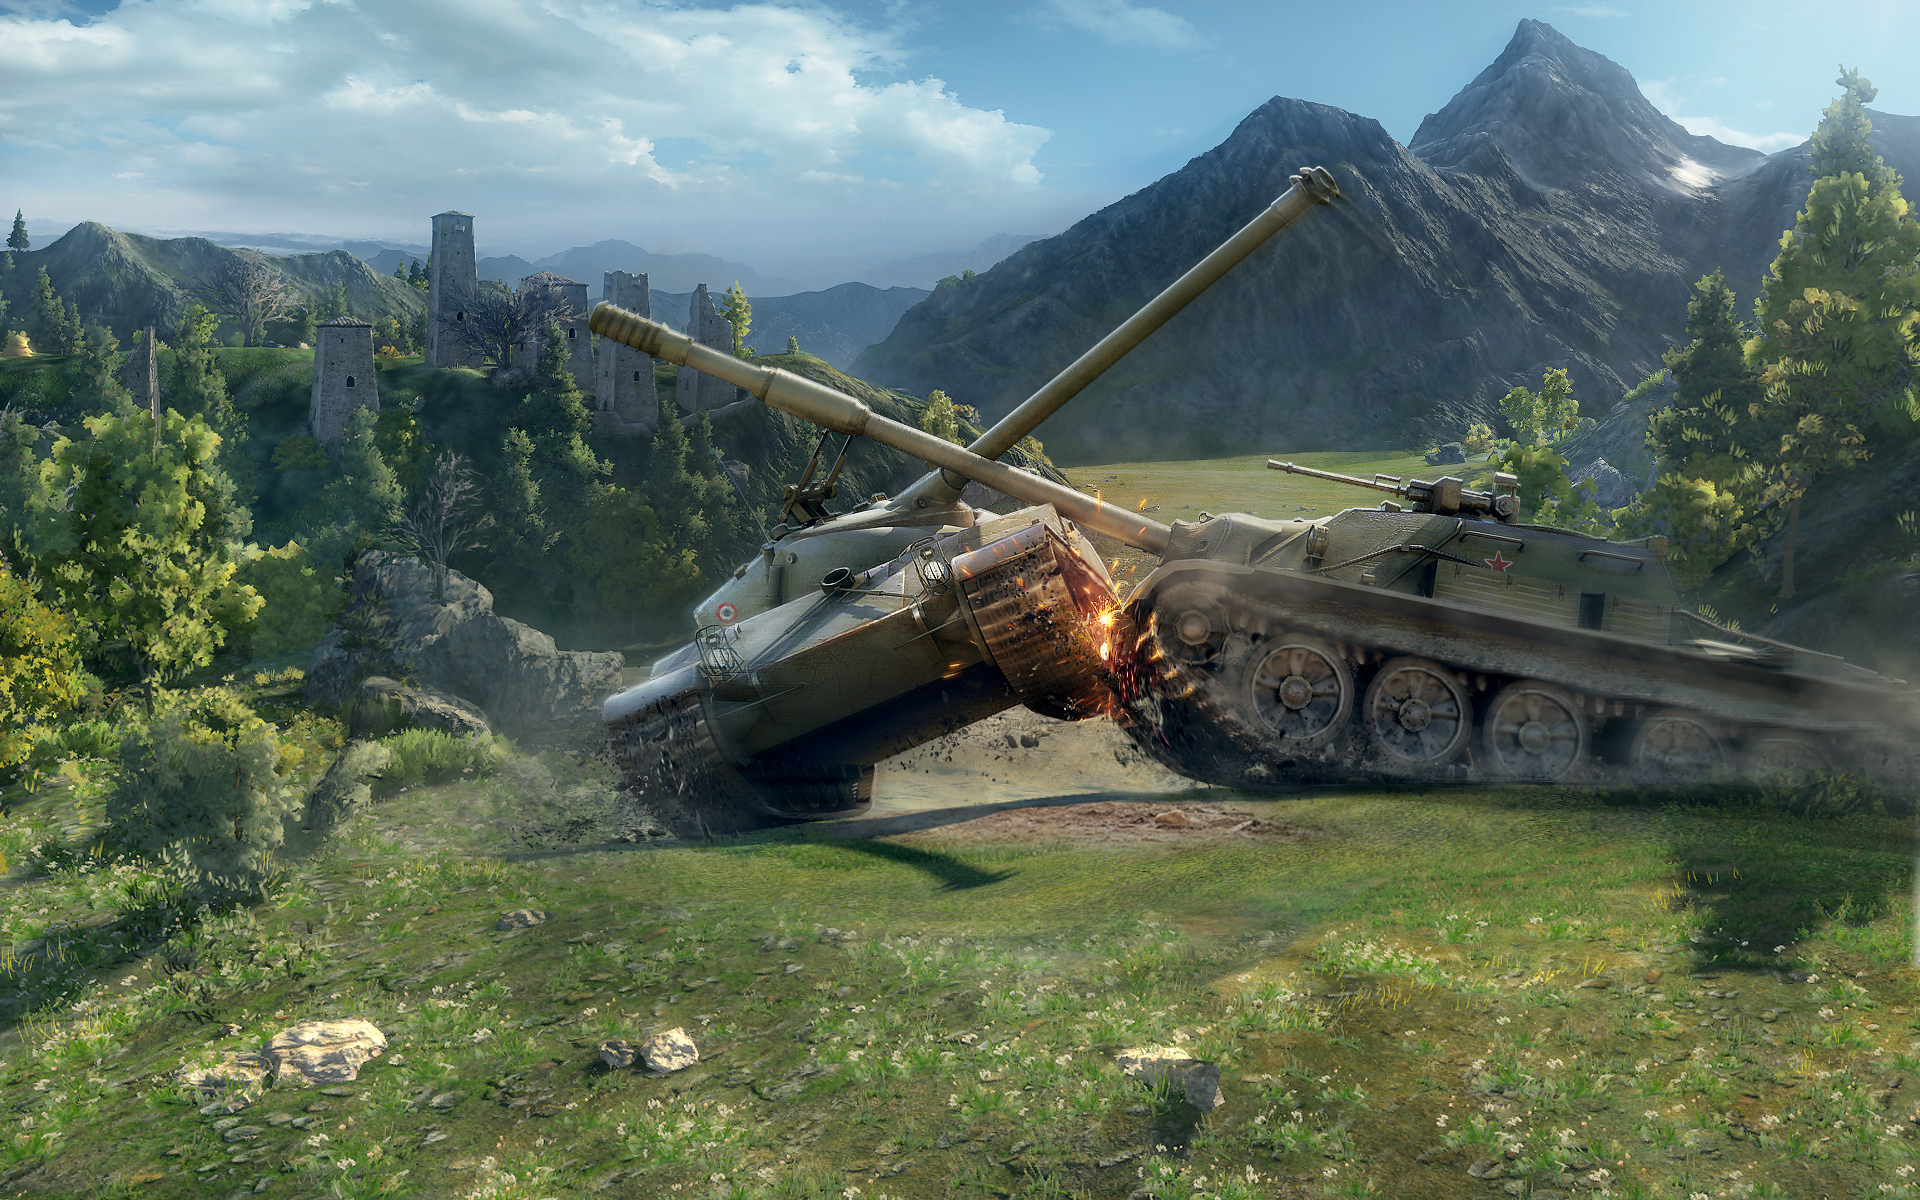
\includegraphics[width=\paperwidth]{wot.jpg}}
\begin{frame}[plain]{}
\end{frame}
}

\begin{frame}{ИДЕИ}
    \begin{itemize}
        \item главное --- скорость и простота разработки
        \item не стоит боятся гетерогенной среды
        \item синхронный подход везде где можно
        \item асинхронный --- только там, где это необходимо
        \item AMQP --- отличный протокол для реализации RPC
        \item работа с объектами в памяти самая быстрая
    \end{itemize}
\end{frame}

{
\setbeamertemplate{footline}{}

\setbeamercolor{frametitle}{fg=white}
\setbeamercolor{normal text}{fg=white}
\setbeamercolor{block title}{fg=white}
\setbeamercolor{block body}{fg=red}
\logo{
    
\includegraphics[height=1.7cm]{wg-logo.png}
}

\usebackgroundtemplate{
\includegraphics[height=\paperheight]{wg-end.jpg}}
\begin{frame}{СПАСИБО ЗА ВНИМАНИЕ. ВОПРОСЫ}
    \begin{block}{Максим Мельников}
    \par \url{mailto:m\_melnikau@wargaming.net}
    \par \url{https://plus.google.com/+MaksimMelnikau}
    \par \url{https://twitter.com/max\_posedon}
    \par \url{http://wargaming.com}
    \end{block}
\end{frame}
}

\begin{frame}{ОСНОВНАЯ ИГРОВАЯ БАЗА}
    \begin{itemize}
        \item размер базы: 300 GB
        \item 384 GB RAM
        \item Percona 5.5 (разогрев кэша --- 1GBps)
        \item 40k select-ов, 1k insert-ов, 1k update-ов в секунду
        \item 24 HDD $*$ 600 GB $*$ 0.5 = 6 TB
    \end{itemize}
\end{frame}

\end{document}

